\documentclass{styles/main}
\usepackage{pgfplots}


\title{\textbf{统计学与概率}}
\author{TechX 人工智能与机器学习课程筹备组}
\date{}


\begin{document}

\maketitle
%\tableofcontents
%\newpage


\section{统计}

统计学作为一门关于数据的科学,在机器学习领域中拥有非常重要的地位。事实上,在早期算力水平远不足如今的时候,所谓的``机器学习''模型和算法都是一些来自于统计学的模型和算法,如线性回归、逻辑回归等等。即便是今天,我们也能在很多机器学习和深度学习的模型和算法背后看到统计学的影子。

首先,我们需要了解统计学中的两个基本概念:\term{样本}与\term{总量}。在现实生活中,当我们想要研究某一组数据时,我们往往不能够将那组数据收集齐全。比如说,如果我们想研究上海美本申请者的托福成绩,我们不可能一个都不遗漏都收集到每一个上海美本申请者的托福成绩,我们只能退而求其次,收集尽可能多的托福成绩。在这种情况下,我们所收集到的所有数据的集合就叫做``样本''(Sample),而样本是``总量''(Population)——即所有上海市美本申请者的托福成绩——的一部分。也就是说,总量是我们想要研究的数据的总体,而总量中的任何一部分数据,不论多少,都可以被称之为该总量的样本。

一般来说,统计学可以被分为\term{描述统计学}和\term{推论统计学}两种。前者注重于描述与总结已有的数据(也就是说收集到的样本)的信息,而后者则注重于从样本中推断出总量的特征。还是拿刚才的例子:比如我们收集到了 1000 个上海市美本申请者的托福成绩,那么我们可以借助描述统计学的工具来总结这 1000 组数据的平均值、最大值、最小值等等信息。但如果我们希望通过这 1000 组数据去推断关于全上海市所有美本申请者的托福成绩,那就是推论统计学的范畴了。

接下来,我们将简单介绍描述统计学中的一些常用的概念。


\subsection{中心值的计算}

  描述统计学的强大之处之一就是我们能用极少的信息来总结较多数据的特征或基本信息。而数据的中心值就是我们最常用的总结数据特征的工具之一。
  
  如果一位教授想知道自己课上所有学生在某一次考试中的表现,除了列出每一个学生的成绩并一一查看,一个更有效且更有用的方法是求出所有成绩的\term{平均值}(Mean)并直接根据其高低判断那门课的学生的总体表现。这一概念想必大家都非常熟悉,如果我们有 $n$ 个数据,分别记为 $x_1, x_2, \dots, x_n$,那么这些数据的平均值(约定俗成记为 $\mean{x}$)就是\footnote{严格地来说,其实有几种不同的平均值,但我们在这里使用``平均值''一词时讨论的永远是算数平均值(Arithmetic Mean)}
  \[ \mean{x} = \frac{x_1 + x_2 + \dots + x_n}{n} \]
  
  平均值是中心值的一种描述,但并非是描述数据中心值的唯一度量。平均值虽常用并极其有效,但其却有一些弊端。比如说,一组数据的平均值很容易被其中一个很大或者很小的数据影响,并使得计算出的平均值并不能很好地反映一组数据的常态。因此,我们有时也会考虑其他中心值的度量,例如\term{中位数}(Median)是将所有数据按大小排列后位置处于最中间的那个数据,还有\term{众数}(Mode)则是所有数据中出现频率最高的一个数据。


\subsection{离散度的计算}
  
  还是拿刚才考试成绩的数据为例,如果教授不仅想知道所有成绩的平均值,还想知道考的差的学生有多差、好的学生又有多好呢?毕竟哪怕两个班级学生分数的平均值一样,还是可能出现一个班级的成绩都集中在平均值周围,而另一个班级的成绩则极其分散——考得好的人考得很好,考得差的人考得很差。在这里,我们想要知道也就是数据的\term{离散度}——即数据有多``分散''。比如,如果我们的数据是某国家每个人的收入情况,那么这个国家的贫富差距越大,对应的数据的离散度也就越高,反之亦然。
  
  一种简单的离散度的度量是数据的\term{范围}(Range),即数据中的最大值减去最小值。虽然范围计算起来便捷,但其却非常容易被\term{异常数据}(Anomalies,即偏离总体数据很远的数据点)影响,导致最终计算出来的范围过大。
  
  一种更加理想的离散度的度量是能够将所有数据点全都列入考虑的度量,其中最常见的度量则是数据的方差(Variance)。用自然语言描述,一个数据的方差指的是:每个数据与平均值的距离的平方的总平均值。也就是说,如果一些数据离平均值越远,那么距离的平方也就越大,从而导致方差也就越大。用公式来表达,假设一组数据 $x_1, x_2, \dots, x_n$ 拥有平均值 $\mean{x}$,那么这组数据的方差(记作 $\sigma^2$)就是
  \[ \sigma^2 = \frac{1}{n} \sum_{i=1}^n (x_i - \mean{x})^2 \]
  
  之所以方差的记号带有一个平方,是因为有一个在实际应用中更为常见的数据离散度的度量:标准误差(Standard Deviation),记为 $\sigma$,其定义为数据方差的平方根,即,
  \[ \sigma = \sqrt{\sigma^2} = \sqrt{\frac{1}{n} \sum_{i=1}^n (x_i - \mean{x})^2} \]



\newpage
\section{概率}

概率这一概念相信大家或多或少地都接触过一些。我们知道概率描述的是某一个事件``多有可能发生'',并且取值范围是闭区间 $[0, 1]$。其中,概率为 1(或者 100\%,两者是相等的)的事件是必然会发生的,而概率为 0(或者 0\%)的事件则必然不会发生。


\subsection{概率的计算}
  
  但只是知道了概率是什么不太够。在不知道一个事件的概率的情况下,我们怎么去计算这个事件发生的概率呢?
  
  例如,给你一枚骰子,你怎么能够计算出投到 6 的概率呢(假设你这一辈子一直生活在山洞里,从来没见过骰子,更不知道这个概率其实就是 $\frac{1}{6}$)?一种方法是自己去投骰子。比如说你投了 10 次骰子,一共投到了 4 次 6,那么你就可以用这两个数据预估出一个投到 6 的概率:

  $$ \textrm{投到 6 的概率} = \frac{\textrm{投到 6 的次数}}{\textrm{总共投的次数}} = \frac{4}{10} = 0.4 $$
  
  不难发现这个概率离真实的 $\frac{1}{6}$ 差得很远。这个简单的例子体现的就是\term{理论概率}与\term{实验概率}的区别。在这里,理论概率之所以是 $\frac{1}{6}$ 是因为我们假设了投到 6 个数字的概率是相等的,且投骰子共有 6 种\term{结果}(Outcome),我们所关注的\term{事件}(Event)只有投到 6 的那个结果。为了加强理解,我们还可以考虑投到奇数的概率。这时,虽然投骰子的结果仍然有 6 种,但我们关注了其中 3 种结果(即投到 1, 3, 或 5)。因此,我们总结得到,如果得到任意结果的概率都是相等的,那么对于某一事件 $A$,其(理论)概率 $\prob(A)$ 为
  
  $$ \prob(A) = \prob(\textrm{得到}\ A\ \textrm{中的某个结果}) = \frac{\textrm{事件}\ A \ \textrm{中的结果数量}}{\textrm{总共的结果数量}} $$
  
\subsection{独立性}
  
  如果我们投两次骰子,那么两次都投到 6 的概率不难得出是 $\frac{1}{36}$。但为什么呢?这背后其实隐藏着我们的一个假设:即两次投骰子的结果是互不干扰,即\textbf{独立}(Independent)的。只有在独立事件间,我们才可以通过简单的概率乘法计算出多个事件获得某个结果的组合的概率。
  
  一般地,对于两个事件 $A, B$,我们称 $A$ 与 $B$ 是独立的当且仅当
  $$ \prob(A \cap B) = \prob(A) \prob(B) $$


\subsection{条件概率}
  
  我们理解了何为一个事件的概率之后,我们再来看什么是条件概率。首先,条件概率也是一个概率,它描述的是一个事件发生的概率如果给定某一事件已经发生了。用符号表达,条件概率 $\prob(A \mid B)$ 描述的是 $A$ 发生的概率如果我们给定 $B$ 已经发生,即,
  $$ \prob(A \mid B) = \frac{\prob(A\ \textrm{与}\ B\ \textrm{都发生})}{\prob(B)} $$
  
%  这一定义可以通过直观的可视化来更好地理解。

  我们还是用上面的投骰子的例子。如果 $A$ 是投到 3 这个事件,且 $B$ 是投到奇数的事件,那么我们不难发现,通过直观推断,如果我们已知 $B$ 发生了,即我们已经投到了 1, 3, 5 中的一个,那么 $A$ 发生的概率并非原来的 $\frac{1}{6}$,而是 $\frac{1}{3}$。
  
  一般地,对于两个事件 $A$ 与 $B$,由于其均是结果的集合,我们可以计算其交集 $A \cap B$(这个交集即 $A$ 与 $B$ 同时发生的事件)那么我们定义条件概率
  $$ \prob(A \mid B) = \frac{\prob(A \cap B)}{\prob(B)} $$
  
  如果对这个概念仍无法直观理解,可以去看一下 \href{https://ocw.mit.edu/resources/res-6-012-introduction-to-probability-spring-2018/part-i-the-fundamentals/MITRES_6_012S18_L02.pdf}{\underline{这个链接}} 里对于条件概率的可视化解释。
  
  注意,我们通过这个定义可以得出一个非常有用的等式:
  $$ \prob(A \cap B) = \prob(B) \prob(A \mid B) = \prob(A) \prob(B \mid A) $$
  
  此外,利用条件概率的定义,我们不难给出一个关于事件独立性的等价的定义,即:事件 $A, B$ 为独立的当且仅当
  $$ \prob(A) = \prob(A \mid B) \quad \textrm{或} \quad \prob(B) = \prob(B \mid A) $$

\subsection{贝叶斯定理}
  
  根据以上对于条件概率的定义,我们能够得出 $\prob(A \cap B) = \prob(A) \prob(B \mid A)$,将这个代入 $\prob(A \mid B)$ 的定义,我们就得到了贝叶斯定理的一种表达方式:
  $$ \prob(A \mid B) = \frac{\prob(A) \prob(B \mid A)}{\prob(B)} $$
  
  \textbf{选做:}可以参考 \href{https://ocw.mit.edu/resources/res-6-012-introduction-to-probability-spring-2018/part-i-the-fundamentals/MITRES_6_012S18_L02.pdf}{\underline{这个链接}} 中对于贝叶斯定理的解释来加深理解。


\subsection{随机变量}
  
  在概率学中,一个\term{实验}(Experiment)指的是一种\term{结果}(Outcome)随机的过程,而一个\term{随机变量}(Random Variable)则是指一个将某实验的每个结果都对应了一个(不一定唯一的)实数的函数。例如,考虑投骰子的实验,那么对应的随机变量可以是投到几就对应到几。此时,这个随机变量的取值范围为 $\set{1, 2, 3, 4, 5, 6}$,且取到每个值的概率都相等。
  
  但是,我们也可以定义一种随机变量,其取值为 1 如果投到的数字是 6,并且取值为 0 如果投到任何其他数字。此时,这个随机变量的取值范围仅为 $\set{0, 1}$,且取到 0 的概率为 $\frac{5}{6}$、取到 1 的概率为 $\frac{1}{6}$,如果我们将这个随机变量记作 $X$,那么我们可以将这两个概率表达为
  $$ \prob(X = 0) = \frac{5}{6},\ \prob(X = 1) = \frac{1}{6} $$
  一般地,我们将一个随机变量 $X$ 取到某值 $x$ 的概率记作 $\prob(X = x)$。
  


%\subsection{概率分布}
%  
%  在统计中,


\subsection{均匀分布}

  最简单也是最容易理解的概率分布就是\term{均匀分布}。均匀分布分为两种:\term{离散均匀分布}与\term{连续均匀分布}。我们这里先只探讨前者。
  
  回到之前提到的投骰子的例子,我们投骰子得到的数值这个随机变量就遵循一个离散均匀分布,因为样本空间中的 6 个可能的结果都拥有相等的 $\frac{1}{6}$ 的概率。一般地,对于一个取值范围有 $n$ 个元素的均匀分布的随机变量,其取到任何一个值的概率都是 $\frac{1}{n}$。
  

\subsection{正态分布}
  
  正态分布是一个在自然界极其常见的概率分布,从人们的身高,正态分布在自然界无处不在。下图中画出了三个不同的正态分布,它们拥有不同的均值和方差。
  
  \begin{figure}[h!]
  \centering
  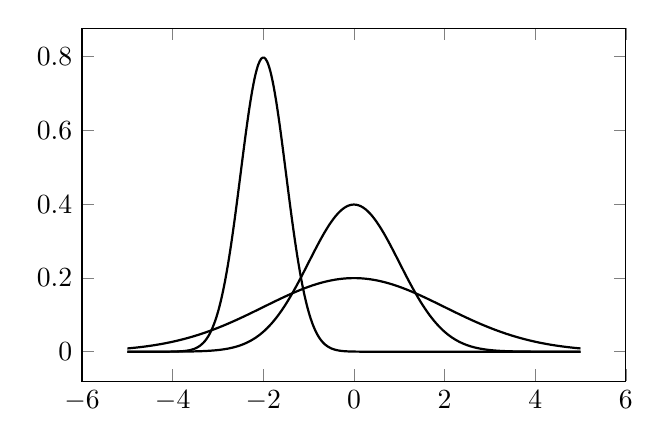
\begin{tikzpicture}
    \begin{axis}[width=.7\textwidth, height=.5\textwidth, legend cell align={left}]
      \addplot[samples=100, smooth, thick]{1/1/sqrt(2*pi) * exp((x-0)^2/(-2 * 1^2))};
      \addplot[samples=100, smooth, thick]{1/2/sqrt(2*pi) * exp((x-0)^2/(-2 * 2^2))};
      \addplot[samples=150, smooth, thick]{1/0.5/sqrt(2*pi) * exp((x+2)^2/(-2 * 0.5^2))};
    \end{axis}
  \end{tikzpicture}
  \end{figure}


\subsection{二项分布}
  
  观看视频:\url{https://www.bilibili.com/video/BV1Bz411b7Jy}。



\end{document}
